\testfile{pgfplotstest.align.tex}
\testsection{Anchors, alignment, baselines, sub nodes}%
\testsubsection{Baseline alignment}
\noindent
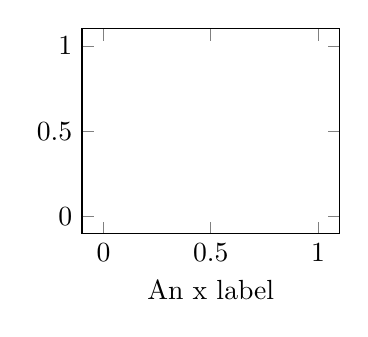
\begin{tikzpicture}[baseline]
	\begin{axis}[width=0.4\linewidth,xlabel=An x label]
		\smallplotstest
	\end{axis}
\end{tikzpicture}
\hspace{1cm}
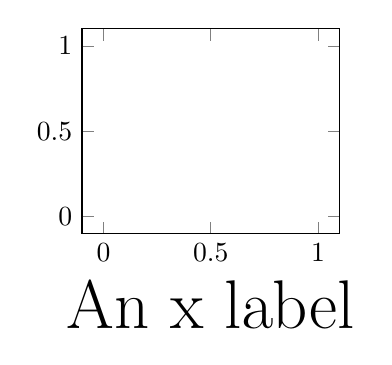
\begin{tikzpicture}[baseline]
	\begin{axis}[width=0.4\linewidth,xlabel={\Huge An x label}]
		\smallplotstest
	\end{axis}
\end{tikzpicture}

\testsubsection{Baseline alignment and externalized graphics}
One needs \texttt{\textbackslash beginpgfgraphicnamed} around the complete paragraph, so this here doesn't work (see source code):

\beginpgfgraphicnamed{baselinetesta}
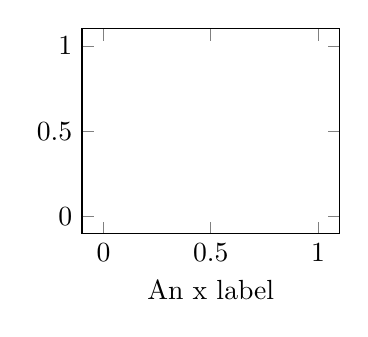
\begin{tikzpicture}[baseline]
\begin{axis}[width=0.4\linewidth,xlabel=An x label]
	\smallplotstest
\end{axis}
\end{tikzpicture}
\endpgfgraphicnamed
%
%
\hspace{1cm}
\beginpgfgraphicnamed{baselinetestb}
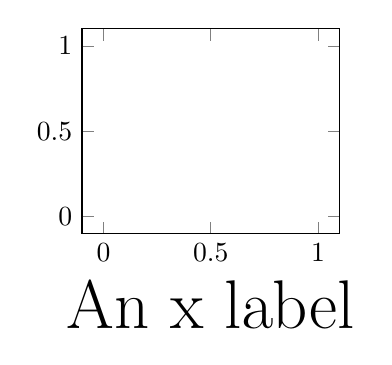
\begin{tikzpicture}[baseline]
\begin{axis}[width=0.4\linewidth,xlabel={\Huge An x label}]
	\smallplotstest
\end{axis}
\end{tikzpicture}
\endpgfgraphicnamed

\testsubsection{Baseline alignment and externalized graphics II}
\beginpgfgraphicnamed{baselinetestc}
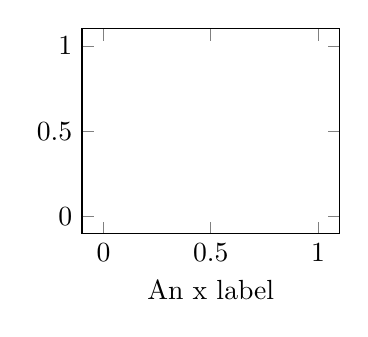
\begin{tikzpicture}[baseline]
\begin{axis}[width=0.4\linewidth,xlabel=An x label]
	\smallplotstest
\end{axis}
\end{tikzpicture}
%
%
\hspace{1cm}
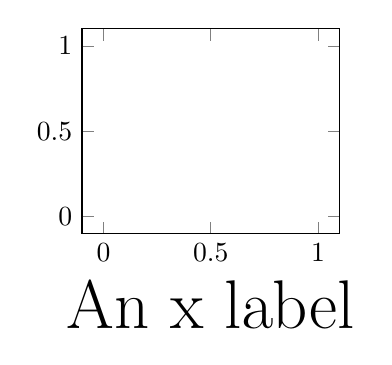
\begin{tikzpicture}[baseline]
\begin{axis}[width=0.4\linewidth,xlabel={\Huge An x label}]
	\smallplotstest
\end{axis}
\end{tikzpicture}
\endpgfgraphicnamed

\testsubsection{Horizontal and Vertical alignment}
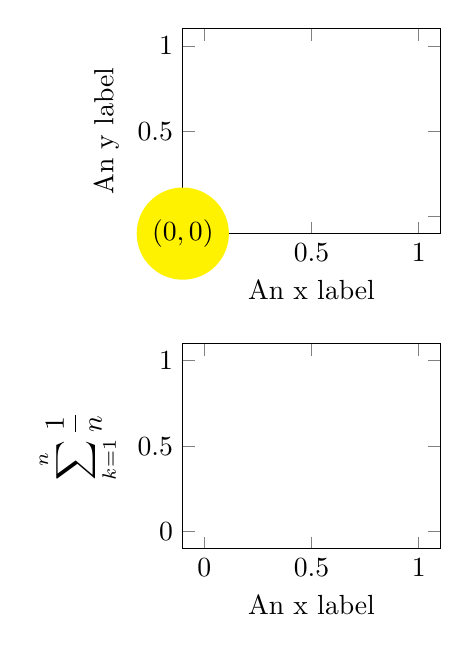
\begin{tikzpicture}[baseline]
\begin{axis}[width=0.4\linewidth,xlabel=An x label,ylabel=An y label]
	\smallplotstest
\end{axis}

\begin{scope}[yshift=-4cm]
\begin{axis}[width=0.4\linewidth,xlabel=An x label,ylabel={$\displaystyle\sum_{k=1}^n \frac 1n$}]
	\smallplotstest
\end{axis}
\end{scope}

\node[fill=yellow,circle] at (0,0) {$(0,0)$};
\end{tikzpicture}
%
%
\hspace{1cm}
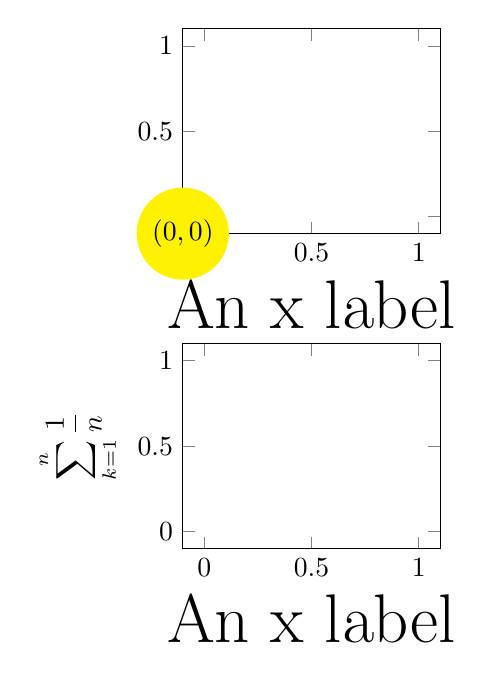
\begin{tikzpicture}[baseline]
\begin{axis}[width=0.4\linewidth,xlabel={\Huge An x label}]
	\smallplotstest
\end{axis}

\begin{scope}[yshift=-4cm]
\begin{axis}[width=0.4\linewidth,xlabel={\Huge An x label},ylabel={$\displaystyle\sum_{k=1}^n \frac 1n$}]
	\smallplotstest
\end{axis}
\end{scope}
\node[fill=yellow,circle] at (0,0) {$(0,0)$};
\end{tikzpicture}

\onecolumn
\testsubsection{Anchortest}
{
	\def\plot{%
	%\tracingmacros=2\tracingcommands=2 % FIXME
		\begin{axis}[
			width=5cm,
			name=test plot,
			xlabel=$x$,
			ylabel={$y$},% = \frac 12 \cdot x^3 - 4 x^2 -16 x$},
			y label style={yshift=-15pt},
			legend style={at={(1.03,1)},anchor=north west},
			title=A test plot.,
			legend entries=$f(x)$,
		]
			\smallplotstest
			%\addplot coordinates {(0,0) (1,1)};
		\end{axis}
	}%
	\def\showplotXX{%
		%\tracingmacros=2 \tracingcommands=2 % FIXME
		\begin{axis}[
			name=test plot,
			axis x line=center,
			axis y line=center,
			enlargelimits=false,
			minor tick num=3,
			tick style={semithick},
			tick align=center,
			xlabel=$x$,
			ylabel=$y$,
			ymin=-0.5,
			xmin=-1.5,
			every axis x label/.style={at={(current axis.right of origin)},anchor=north east},
			every axis y label/.style={at={(current axis.above origin)},anchor=north east},
			inner axis line style={->},
		]
		%\addplot plot[domain=-2:5] (\x,20*\x);
			\smallplotstest
		\end{axis}
	}
	\def\showit#1#2{%
		\node[pin=#2:(s.#1),fill=black,circle,scale=0.3] at (test plot.#1) {};
	}%
	\tikzstyle{every pin}=[opacity=0.5,fill=yellow,rectangle,rounded corners=3pt,font=\tiny]
	\def\TESTPLOTS{%
				\begin{tikzpicture}
					\plot
					\showit{north}{90}
					\showit{north west}{135}
					\showit{west}{180}
					\showit{south west}{225}
					\showit{south}{270}
					\showit{south east}{305}
					\showit{east}{0}
					\showit{north east}{45}
					\showit{center}{90}
				\end{tikzpicture}
				\vskip1cm

				\begin{tikzpicture}
					\plot
					\showit{outer north}{90}
					\showit{outer north west}{135}
					\showit{outer west}{180}
					\showit{outer south west}{225}
					\showit{outer south}{270}
					\showit{outer south east}{305}
					\showit{outer east}{0}
					\showit{outer north east}{45}
					\showit{outer center}{90}
				\end{tikzpicture}

				\vskip1cm
				\begin{tikzpicture}
					\plot
					{\pgfplotsset{every pin/.append style={pin distance=1cm}}%
					\showit{above north}{90}
					}%
					\showit{above north east}{90}
					\showit{right of north east}{0}
					\showit{right of east}{0}
					\showit{right of south east}{0}
					\showit{below south east}{-90}
					{\pgfplotsset{every pin/.append style={pin distance=1cm}}%
					\showit{below south}{-90}
					}%
					\showit{below south west}{-90}
					\showit{left of south west}{180}
					\showit{left of west}{180}
					\showit{left of north west}{180}
					\showit{above north west}{90}
				\end{tikzpicture}

				\vskip1cm
				\begin{tikzpicture}
					\showplotXX
					{\pgfplotsset{every pin/.append style={pin distance=1cm}}%
					\showit{above origin}{45}
					}%
					\showit{right of origin}{45}
					{\pgfplotsset{every pin/.append style={pin distance=1cm}}%
					\showit{below origin}{0}
					}%
					\showit{left of origin}{135}
					\showit{origin}{135}
				\end{tikzpicture}
	}
	%\tracingmacros=2\tracingcommands=2
	%\message{HIER!?}%
	\TESTPLOTS

	\testsubsection{Using non-standard unit vectors}
	{
		\pgfplotsset{every axis/.append style={
				x={(30pt,9pt)},
				y={(-15pt,45pt)},
			}}
		\TESTPLOTS
	}

	\testsubsection{3D}
	{
		\let\smallplotstest=\smallplotstestthree
		%\tracingmacros=2\tracingcommands=2
		\TESTPLOTS
	}

	\testsubsection{Using anchors before axis is finished}
	{
		\def\showit#1#2{%
			\node[pin=#2:(s.#1),fill=black,circle,scale=0.3] at (current axis.#1) {};
		}%
		\def\TESTPLOTS{%
			{
			\pgfplotsset{every axis/.append style={
				extra description/.code={
							\showit{north}{90}
							\showit{north west}{135}
							\showit{west}{180}
							\showit{south west}{225}
							\showit{south}{270}
							\showit{south east}{305}
							\showit{east}{0}
							\showit{north east}{45}
							\showit{center}{90}
				}}}
			\begin{tikzpicture}
				\plot
			\end{tikzpicture}
			}
			{
			\pgfplotsset{every axis/.append style={
				extra description/.code={
					{\pgfplotsset{every pin/.append style={pin distance=1cm}}%
					\showit{above origin}{45}
					}%
					\showit{right of origin}{45}
					{\pgfplotsset{every pin/.append style={pin distance=1cm}}%
					\showit{below origin}{0}
					}%
					\showit{left of origin}{135}
					\showit{origin}{135}
				}}}
			\begin{tikzpicture}
				\showplotXX
			\end{tikzpicture}
			}
		}%
		\TESTPLOTS

			{
			\pgfplotsset{every axis/.append style={
					x={(30pt,9pt)},
					y={(-15pt,45pt)},
				}}
			\TESTPLOTS
			}
	}
}

\twocolumn


\testsubsection{Accessing sub-nodes}
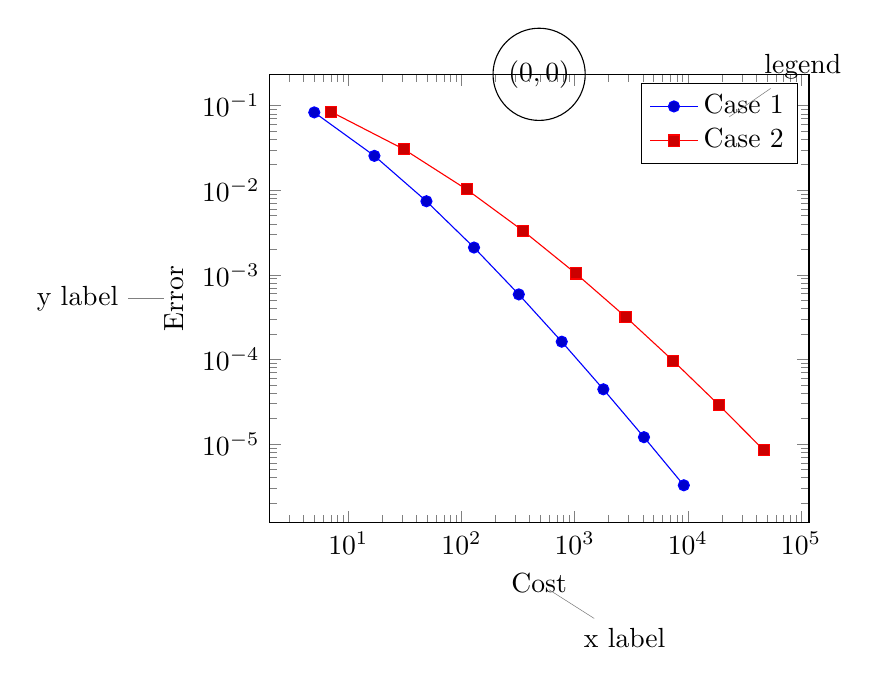
\begin{tikzpicture}[baseline]%
	\node[circle,draw=black] at (0,0) {$(0,0)$};
	\begin{loglogaxis}[
		anchor=north,
		name=firstplot,
		xlabel=Cost,
		ylabel=Error,
		y label style={name=myylabel},
		x label style={name=myxlabel},
		legend style={name=mylegend,
			row 1 column 2/.style={blue,name=firstentry}% doesn't work!
		}
	]
	\addplot plot coordinates {
		(5,     8.31160034e-02)
		(17,    2.54685628e-02)
		(49,    7.40715288e-03)
		(129,   2.10192154e-03)
		(321,   5.87352989e-04)
		(769,   1.62269942e-04)
		(1793, 4.44248889e-05)
		(4097, 1.20714122e-05)
		(9217, 3.26101452e-06)
	};
	\addplot plot coordinates {
		(7,     8.47178381e-02)
		(31,    3.04409349e-02)
		(111,   1.02214539e-02)
		(351,   3.30346265e-03)
		(1023,  1.03886535e-03)
		(2815,  3.19646457e-04)
		(7423,  9.65789766e-05)
		(18943, 2.87339125e-05)
		(47103, 8.43749881e-06)
	};
	\legend{Case 1\\Case 2\\}
	\end{loglogaxis}

	\node[pin=45:legend] at (mylegend.center) {};
	\node[pin=-45:x label] at (myxlabel.center) {};
	\node[pin=180:y label] at (myylabel.center) {};
\end{tikzpicture}%

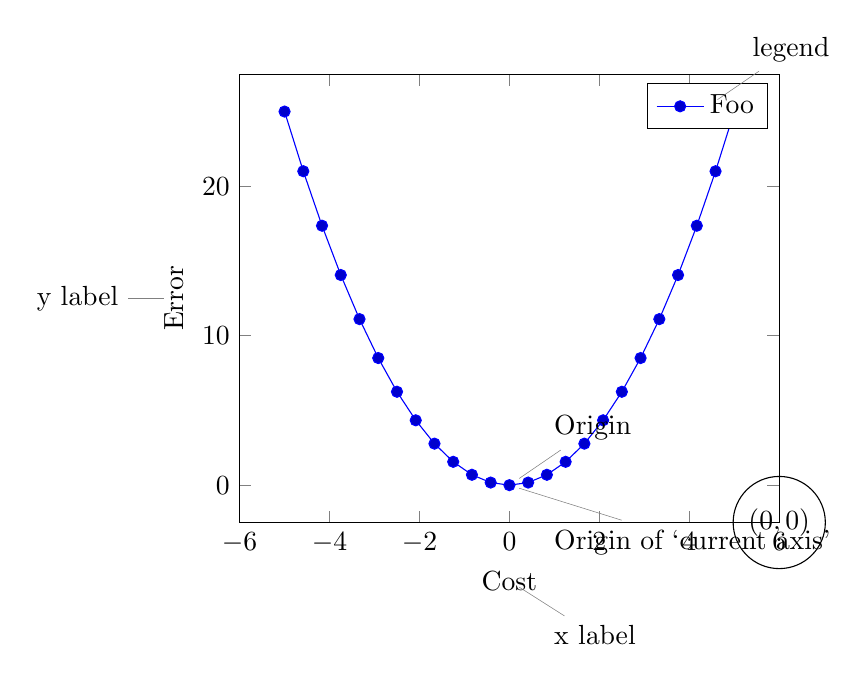
\begin{tikzpicture}[baseline]%
	\node[circle,draw=black] at (0,0) {$(0,0)$};
	\begin{axis}[
		anchor=south east,
		name=firstplot,
		xlabel=Cost,
		ylabel=Error,
		y label style={name=myylabel},
		x label style={name=myxlabel},
		legend style={name=mylegend,
			row 1 column 2/.style={blue,name=firstentry}% doesn't work!
		}
	]
	\addplot (\x,\x^2);
	\legend{Foo}
	\end{axis}

	\node[pin=45:legend] at (mylegend.center) {};
	\node[pin=-45:x label] at (myxlabel.center) {};
	\node[pin=180:y label] at (myylabel.center) {};

	\node[pin=45:Origin] at (firstplot.origin) {};
	\node[pin=-45:Origin of `current axis'] at (current axis.origin) {};
\end{tikzpicture}%


\testsubsection{Funny bounding boxes}
\testsubsubsection{(my plot.below south west) rectangle (my plot.above north east)}
{
The following figure is centered:
\setlength{\fboxsep}{0pt}%
\begin{center}
\fbox{%
\begin{tikzpicture}%
	\begin{pgfinterruptboundingbox}
	\pgfplotsset{every axis legend/.append style={at={(1.03,1)},anchor=north west}}
	\begin{axis}[
		name=my plot,
		title=A title,
		xlabel={\Huge An x label},
		ylabel={$\displaystyle\sum_{k=1}^n \frac 1n$}
	]
		\smallplotstest
		\addlegendentry{My plot}
	\end{axis}
	\end{pgfinterruptboundingbox}

	\useasboundingbox (my plot.below south west) rectangle (my plot.above north east);
\end{tikzpicture}%
}%
\end{center}
}
